\begin{figure*}[t!]
	\begin{center}
		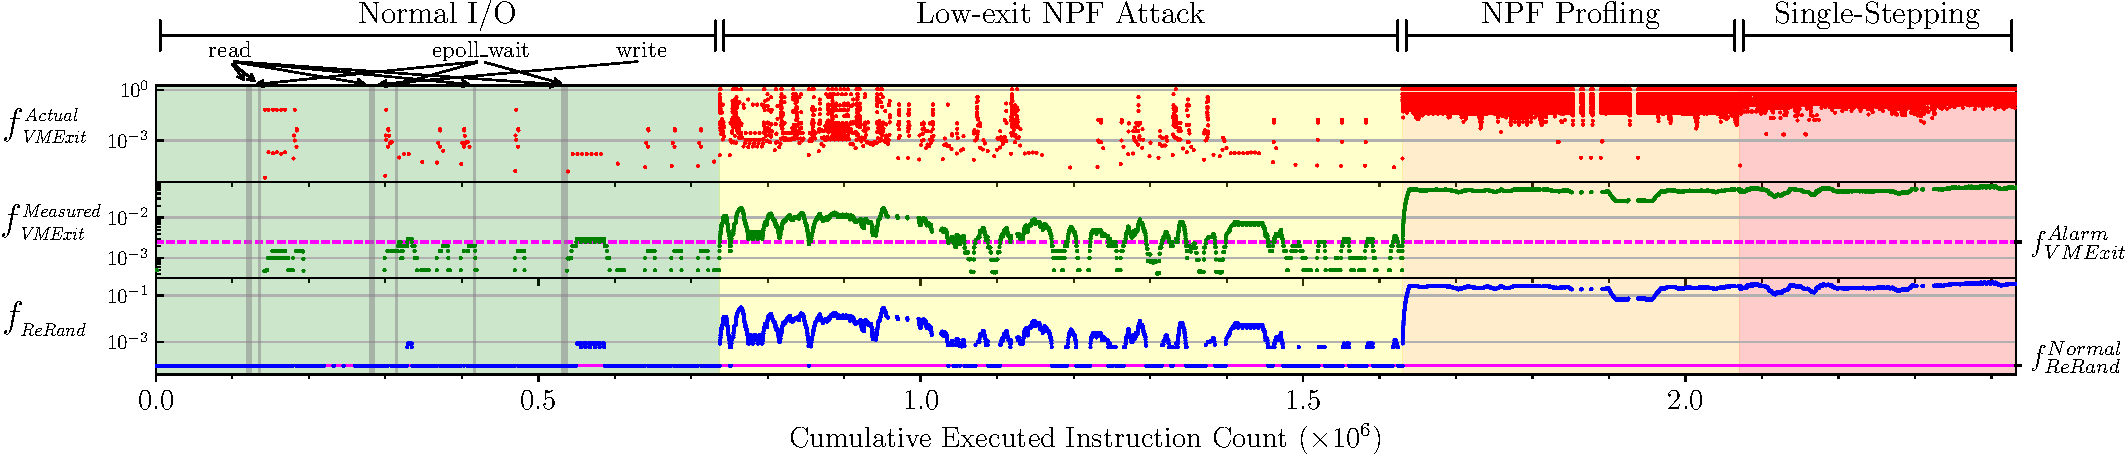
\includegraphics[width=.98\textwidth]{figures/incognitos/adaptive-rerand-final.pdf}
	\end{center}
	\caption{
		VMExit frequencies measured by \thename vs. ground truth (in-KVM), and the resulting adaptive randomization rates for Redis under various workloads and attacks.
		% \thename-measured and ground truth (obtained in-KVM)  VMExit frequencies and the adaptive randomization frequencies of a running Redis server under different workloads and attacks.
	}
	\label{fig:eval-adaptive-rerand}
	% \lnginx, \llenpf, \lnpf, \lss (\autoref{tab:attack-exit-rates})}
\end{figure*}

\section{Evaluation}
\label{sec:incog:evaluation}

In this section, we evaluate \thename in terms of its security and performance feasibility through six experiments: 1. robustness of VMExit frequency measurement (\cref{subsec:robustness-eval}), 2. access pattern profiling resilience in NGINX (\cref{subsec:profiling-attack}), 3. LibJPEG image extraction attack mitigation (\cref{subsec:jpeg-attack}), 4. \nbench microbenchmark (\cref{sec:eval:microbench}), and real-world application performance benchmarks (\cref{sec:eval:real-app}) with 5. NGINX and 6. Redis.
We provide a qualitative security discussion in \cref{sec:sec-ana}.


\hdr{Implementation}
\thename is implemented as a fork of the Unikraft unikernel version v0.15.0~\cite{unikraft-0.15}.
The kernel was modified to support whole-VM memory encryption and mapping integrity protection during boot, along with \gls{ghcb}-based communication with the hypervisor~\cite{amd64}.
Additionally, the networking stack was updated for compatibility with the SEV-aware \texttt{virtio} driver.
$3,401$ lines of code were added or modified for SEV-SNP compatibility, not including \thename's design elements.
We implemented \thename's kernel component in $9,427$  lines of code and its binary rewrite in 682 lines as a plugin to the \texttt{e9patch} binary instrumentation framework~\cite{e9patch}.


% \key{Porting Unikraft to run in a SEV-SNP \gls{cvm} required significant changes.}

% We also modified Unikfraft to place the entire VM memory under SEV-SNP's VM memory encryption and mapping integrity protection during boot according to the specifications~\cite{amd64}.

% \limcomm{Emphasize our engineering efforts here? 1) We ported Unikernel for SEV 2) LoC of our impl.}{*}
% Regarding security, we evaluate the robustness of \thename's dynamic rerandomization rate regulation mechanism against the attack primitives (\cref{subsec:rate-adaptive-eval}) and the effectiveness of its randomization in terms of data access pattern against practical attacks (\cref{sec:eval:attack}).
% We analyze \thename's performance characteristics and its impact on real-world workloads through microbenchmarks (\cref{sec:eval:microbench}) and benchmarks with real-world applications (\cref{sec:eval:real-app}).

\hdr{Experiment environment}
The evaluation is performed on a server equipped with AMD EPYC 7513 CPU@2.0GHz (AMD SEV-SNP capable) and 256GB of RAM, running Ubuntu 22.04 with kernel version 6.9.0-rc.
Also, the experiments used SEV-supported QEMU (commit hash \texttt{bf83c1b9}) and OVMF (commit hash \texttt{80318fcd}) versions provided by AMD.
We have also taken measures to reduce variances during the benchmarks.
For all experiments, the QEMU process and the benchmarking program (e.g., \texttt{ab}) are pinned to dedicated cores (e.g., \texttt{taskset -c 4}) that are reserved at boot (using \texttt{isolcpus} kernel parameter).


\hdr{Parameter settings} {All parameters to \thename's policy are applied as described in \cref{subsec:policy-parameters}}.
However, note that we disabled the grace period mechanism by setting $G=0$ to fully illustrate the effects of rerandomizations for the experiments in \cref{subsec:rate-adaptive-eval}, \cref{subsec:profiling-attack}, and \cref{subsec:jpeg-attack}.
The following table summarizes the parameters that were used, which also includes the ORAM configurations:
% As to the parameterizations for ORAM we also used the same settings as described in \cref{subsec:oram-page-pool}.

% We choose $Z = 4$ and set the stash size to a generous number $S = 512$ to avoid too frequent background evictions~\cite{ren2013design}.
% A static ORAM tree size of 512MB supports all tested workloads.
% \vspace{0.3em}
\begin{table}[h]
	\setlength\tabcolsep{3pt}
	\renewcommand{\arraystretch}{0.3}
	\footnotesize
	\centering
	\begin{NiceTabular}{cccccccc}[corners]
\toprule
 \multicolumn{5}{c}{\thename Parameters } &
 \multicolumn{3}{c}{ORAM Params.} 
 % \Block[p{3cm}]{1-3}{\thead{ORAM parameters (\cref{subsec:oram-page-pool})}} &&  
 \\
\cmidrule(lr){1-5}
\cmidrule(lr){6-8}
\actrg{} Size& $W$ & \freqvmexitof{Alarm}& \freqrrof{Normal} & $G$   & $N$ & $S$ & $Z$ \\ 
\midrule
\makecell{$8,192$\\(32MB)}&
% 123&
$100$ &
$0.003$ &
$\frac{1}{10K}$ $\sim$ $\frac{1}{2M}$ &
$1000$ &
\makecell{$32,768$\\(128MB)}&
% \Block{1-1}{$32,768$\\(128MB)} &
$512$ &
$4$\\
\bottomrule
\end{NiceTabular}
\end{table}
\

\subsection{Robustness evaluation}
\label{subsec:rate-adaptive-eval}
\label{subsec:robustness-eval}
We evaluated the robustness of \thename adaptive rerandomization scheme with \thename-hosted Redis, as shown in ~\autoref{fig:eval-adaptive-rerand}.
The graph allows us to evaluate how close \thename's VMExit frequency measurements (\freqrrofof{\textit{VMExit}}{\textit{Measured}}) and rerandomization rate (\freqrrofof{\textit{ReRand}}{})  approximate the ground truth VMExit frequency measurements (\freqrrofof{\textit{VMExit}}{\textit{Actual}}).



% in sequence to put \thename's VMExit frequency measurement system to the test.

% We ran an instance of \thename-hosted NGINX web server.
\hdr{Measurement method}
The data points of the in-hypervisor framework mentioned in \cref{subsec:empirical-analysis} (ground truth) and \thename are synchronized at each of \thename's ticks.
At each invocation, the scheduler reports its VMExit frequency and rerandomization rate to the framework via a custom hypercall excluded from the VMExit counts.
% \limcomm{Correct? From my understanding, the ground truth is evaluated separately.}{In response}, the framework would calculate and record the ground truth VMExit frequency, along with the reported data from \thename.
% % \khacomm{Shortened}{}
% \limcomm{Too many 'measure...', and what's the purpose of this sentence?}{Therefore, all data points in the graph capture the ground truth measurement and \thename's measurements.}


\hdr{Experiment setup}
% For the experiment, we deployed an instance of \thename-hosted Redis in-memory data store.
We applied 1) normal I/O workload, 2) low NPF controlled-channel attack, 3) conventional NPF controlled-channel attacks, and 4) single-stepping (\lredis, \llenpf, \lnpf, and \lss from \autoref{tab:attack-exit-rates}) to the CVM in a sequence, whose intervals are labeled with \emph{Normal I/O}, \emph{Low-exit NPF Attack}, \emph{NPF Profiling}, and \emph{Single-Stepping} in the graph, respectively.
The initiation of the attacks was synchronized with Redis's \texttt{accept} system call that signifies the beginning of Redis request handling.
The low NPF controlled-channel attack targets specific pages that give away information and, therefore, are program-specific.
Thus, we first profiled the working set (i.e., frequently accessed pages), then randomly chose 10\% of the pages to be monitored to emulate the effect of the attack.
%We invalidated all pages once for the evaluation, then monitored 10\% % of NPF traces collected from the initial invalidation to sustain exit rates throughout the attack.

% While the sequences were executing, we measured the \emph{ground truth} VMExit frequency using the in-hypervisor measurement framework from \cref{subsec:empirical-analysis}, and \thename's \emph{measured} VMExit frequency and applied rerandomization frequency.

% Synchronization

\iffalse
	% Workload and Attacks
	Our goal is to obtain the \emph{trace} of measured and actual VMExit rate throughout the execution of the workload/attacks for comparative analysis.
	Thus, the ground truth measured within the hypervisor and the in-CVM measurement sampled by \thename's scheduling subsystem must be synchronized.
	To do this, the measurement framework maintains a running log that consists of samples of 1) the instruction execution timestamp (sampled from the PMU), 2) the exit code  VMExit that occurred, and 3) the argument of the VMExit.
	The trace is appended with a new sample at every VMExit handling.
	Based on 1), we may calculate the ground truth VMExit frequency at each exit (reciprocal of instructions executed between each exit).
	% Since sampled BB sizes are not fully accurate
	% We used the executed instruction count sampled from the PMU as the ground truth for execution.
	% At each VMExit handling, we log the number of retired instructions, as well as the VMExit reason and its argument (e.g., \texttt{\{ins: 50, exit_code: 0x800000701, arg: 0x0\}}.
	% This is the basis for calculating the ground truth VMExit rate (1/.
	At each scheduler invocation, after the \freqvmexit{t} and \freqrrof{t} are calculated, the values are reported from the CVM to the in-KVM framework as an argument to custom hypercalls.
	This instance of VMExit is appended to the running trace by the measurement framework.
	After our offline analysis of the trace identifies the custom hypercalls and synchronizes them with the timestamp of the ground truth exit rate.

\fi

% Thus, the hypercal
% When the in-KVM measurement framework receives this hypercall, it adds the values to the ongoing trace of ground truth/measured VMExit, recording them at the current timestamp.
% It add these values to the internal log .






% To synchronize the ground truth 




% 1) the executed instruction counts at each VMExit and is used to calculate \emph{groundtruth} VMExit frequencies (labeled \textbf{\emph{Actual Exit Rate}} in the figure), 

% 2) the \emph{measured} VMExit frequency (\textbf{\emph{Measured Exit Rate}}) and 

% 3) the adapted rerandomization rate (\textbf{\emph{ReRand. Rate}}).

% For the first, we sampled their traces using the 
% As for the second and third, we inserted probes in the scheduling function to report the values to the measurement framework through a custom hypercall.
% Note that the VMExit from reporting hypercall itself was excepted from measurement.
% The measurement framework then logged all the samples into a file for offline analysis.

% On the instance of the Redis server, we used the local \texttt{redis-benchmark} to send \emph{four} \texttt{GET} requests and recorded the values mentioned above during the intervals that Redis is serving the request,  starting from the \texttt{accept4} system call and ending at the \texttt{close} system call.
% Each interval is represented with a different color on \autoref{fig:eval-adaptive-rerand}.
% The first interval is designated to represent the normal CVM I/O workloads (\lredis in \autoref{tab:attack-exit-rates}).
% For the subsequent intervals, we introduced attack workloads with increasing VMExit frequencies (\llenpf, \lnpf, and \lss also from \autoref{tab:attack-exit-rates}).





% we  and recorded measurements from \emph{four} 

% We then used a local \texttt{redis-benchmark} client to perform a single \texttt{GET} request to Redis and obtain the samples for the workloads (\lredis from \autoref{tab:attack-exit-rates}).
% Also, we launched side-channel attacks scenario, \llenpf, \lnpf, and \lss from \autoref{tab:attack-exit-rates}.

% Redis is handling requests (which is identified to be in between two \texttt{accept} system calls.



% \textcolor{red}{are performed in the intervals  XX and XX XX respectively}.
% The results from this 


% Then, we applied workloads on the key-value store (\lnginx from \autoref{tab:attack-exit-rates}) using a local \texttt{redis-benchmark} client

% from \hjcomm{When does it start and when does it end?}{\textcolor{red}{intervals labeled L2, L3, etc..}}.


\hdr{Result discussion}
% \jycomm{We should cut end of NPF. I think it is just lopping in a while loop because the socket is closed -> leading to low NPs. Should we mention these issues in continuous high exit scenarios it may be infeasible for application to run? + argue that this is not a usual case for attacks? + additional overhead due to our hypercall based profiling}{}
Overall, the result in the graph confirms the robustness of \thename's VMExit frequency measurement.
We found the following observations to be noteworthy:

First, the results show that \thename suppresses the rerandomization frequency during benign workloads while
promptly reacting to the attacks to fight them with a very high rerandomization frequency.
When the ongoing attack is absent, \freqrrof{Normal} is mostly maintained with minor spikes.
However, \thename showed drastically higher frequency (\freqrrof{Alarm}) applied to low exit NPF, conventional NPF, and single-stepping.
More specifically, the average randomization frequencies were adjusted to be about $0.003$, $0.2007$, and $0.245$ on average, respectively (i.e., once rerandomization every 333, 4, and 5 instructions).
$93.8\%$ of ticks triggered alarmed frequencies of rerandomization, even with the low-exit NPF attack.
This number increases to $100\%$ for NPF profiling and single-stepping attacks.
% perspectively, meaning a rerandomization is scheduled at almost every tick.
% \jycomm{Same for the NPF}{Notably, a constant maximum rerandomization frequency is applied to the single-stepping scenario.}
% Also, while disabled for the experiment, \thename's grace period termination policy 
% the result shows that with the chosen \freqvmexitof{Alarm} threshold, \thename can reliably differentiate between benign and attack scenarios, keeping the rerandomization overheads low while promptly responding to attacks.
% During the benign workload execution (\lnginx interval), the randomization rate remained steady at the configured \freqrrof{Normal} (once every $10,000$ instruction).
% Beginning with the low exit rate NPF attack (\llenpf), the randomization rate is adjusted proportionally to the measured VMExit rate once every.

Second, \thename reliably handled the VMExit frequency spikes during the benign workloads.
If an instantaneous decision was to be made with a fixed threshold, these could have been mistaken for an attack.
We manually confirmed that these spikes occurred during I/O activities.
We marked the locations of spikes with identified sources on the timeline by labeling invoked system calls, such as \texttt{read} and \texttt{write}, on the timeline.
% \khacomm{Mention that their peaks are similar to low NPF}{*}
\thename handled the spikes with momentarily alarmed rerandomization frequency enforcement, yet the execution continued.
% \khacomm{check}{.}
% More specifically, we observed only \textcolor{red}{$0.8\%$} of ticks entered an alarmed state during 

\iffalse
	Lastly, while the measured VMExit frequency closesly approximates that of the ground truth, inherent fluctuations occurred.
	\hjcomm{Where are the fluctations? Also we need denser x-axis lables}{For instance, one such fluctuation can be seen at \textcolor{red}{xx} and \textcolor{red}{xx}, and similar patterns appear in multiple places.}
	These fluctuations can be explained by the instruction count that differs from one basic block to another.
	Hence, \thename's per basic block ticks inevitably cause distance variances between the data points.
	Nevertheless, the results show that \thename's per-basic block tick placement strategy is still robust.
\fi
% Observation 1) There are fluctuations in the measured VMExit rates, probably due to the difference in basic block sizes.



% The spikes in benign workload execution would potentially introduce false-positive cases in a threshold-based termination policy

% while in the case of \thename's, there would only be a temporary surge in the rate of memory rerandomization. 

% This confirms the advantages of using the \thename adaptive scheme.




% Observation 2) There are spikes of VMExit even in normal workloads that are close the rate of attacks -> would have false alarm if not for adaptive rerand. Higher thresholds would have missed the low exit attack case.

% 3) with the chosen threshold \freqvmexit{Alarm}, \freqrrof{Alarm} is engaged very closely to the attacks.
% - While there are spikes in normal workload,


% 1) There are spikes of VMExit even in normal worklodas

% shows the robustness of \thename's VMExit frequency measurement system.
% \thename's measured VMExit frequency (green line graph) closely matches the actual VMExit frequency changes for the most part.


% During this, we ob








\subsection{Access pattern profiling resilience }
% \label{sec:sec-ana:attack}
% \label{sec:eval:attack}
\label{subsec:profiling-attack}
The NGINX memory address profiling attack experiment demonstrates \thename's resilience to code data access profiling attacks (\cref{sec:relatedwork:profiling}).
\autoref{fig:profiling-attack} presents the profiling results of two versions of \thename-hosted NGINX web servers: one without randomization, whose observable traces are shown with the label {\emph{Without Rerand}}, and one with \thename's rerandomization policy (\emph{With Rerand}.
% (\textcolor{blue}{blue} dot graph, \emph{Rerand Freq.})  approximate the ground truth VMExit frequency measurements (\textcolor{red}{red} dot graph, \emph{Actual VMExit Freq.})

\hdr{Experiment setup}
We adapted the technique from a previous work that performed a profiling attack on a \texttt{OpenSSH} server~\cite{heckler} to a \thename-hosted NGINX.
The attack traces the \gls{cvm}'s page access patterns through the \gls{npf} controlled channel and
computes the \gls{cvm}'s \emph{access frequency} for each unique \gls{gpa} page based on the trace.
% This information can be utilized to determine which functions or data structures correspond to each page through statistical analysis.
% \limcomm{Necessary?}{Since \texttt{OpenSSH} is not available on Unikraft,} we instead profiled the page access trace of the NGINX web server serving HTTPS requests.
Both web servers are configured to use the active regions with identical sizes (8,192 slots) for a more accurate comparison.
% except that active regions of \emph{Without Rerand} are not rerandomized.}
% version are not applied with adaptive rerandomization.
% Note, the window where profiling is performed matches the interval labeled L5 in} \autoref{fig:eval-adaptive-rerand}.
% For better comparison, for both 

% with tests on both an unprotected server and one with \thename's protection.
\begin{figure}[t]
	\begin{center}
		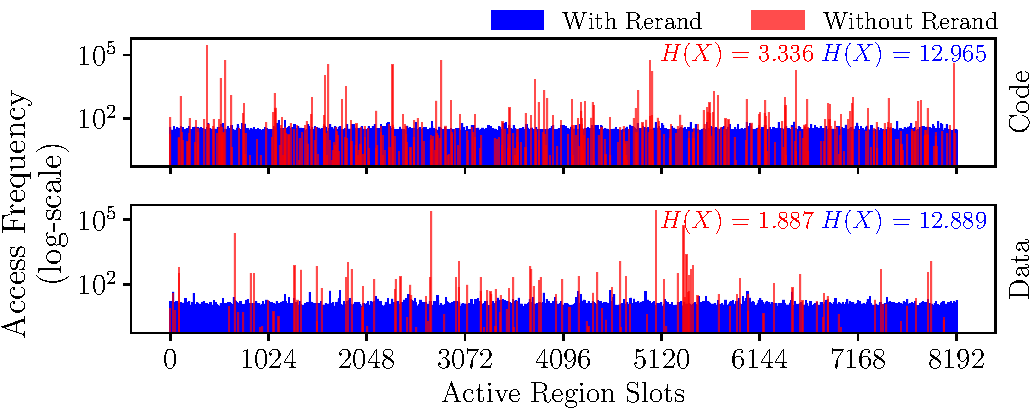
\includegraphics[width=.98\columnwidth]{figures/incognitos/profiling.pdf}
	\end{center}
	\caption{NPF controlled-channel profiling results of \thename-hosted NGINX code and data page access frequency during single HTTPS request.
		$H(X)$ values show Shannon entropy values.}
	\label{fig:profiling-attack}
\end{figure}

\hdr{Result discussion}
The results show that performing \gls{npf}-based profiling is highly infeasible against \thename's adaptive rerandomization.
During the entire attack duration, an average \freqrrof{Alarm} of {0.2} was observed, triggering a rerandomization at almost every tick.
Each rerandomization would render the attack meaningless since each physical page will take a random position (out of 8,192 slots) after the rerandomization.

In the case of \emph{Without Rerand}, the page access patterns reveal distinct profiles during request handling (max~$= 289,995$/$237,372$, mean~$= 82.94$/$67.48$, std.~$= 3471.95$/$3684.0$ for \actrg{code}/\actrg{data}).
This quintessential access frequency pattern allows the adversary to narrow down or pinpoint the sensitive pages.
On the other hand, the \emph{With Rerand} histogram illustrates the effect of elevated rerandomization rate, which shows the collected profile approximating a uniform distribution, where only slight variations are observed (mean~$ = 24.14$/$7.78$, std.~$= 5.61$/$3.24$ for \actrg{code}/\actrg{data}).

To further validate the results, we computed the \emph{Shannon entropy} for each histogram that quantifies the unpredictability of page accesses to each active region slot.
High entropies of $H(X) = 12.965$ for code and $12.889$ for data were observed for the constantly rerandomized NGINX, which translates to roughly $2^{13} = 8,192$ all possible page locations, meaning that the page access patterns are indistinguishable.

% \limcomm{Hard to understand, Why did you computed the \emph{Shannon entropy}? and what it is?}

% }



% to occur on a specific page in this context


% for each memory access.

% while in its worst cases




\subsection{Thwarting JPEG image extraction attack}

% \hdr{JPEG image extraction mitigation}
\label{subsec:jpeg-attack}
% With the LibJPEG attack example (\autoref{fig:jpeg-attack}), we performed a real-world image reconstruction attack~\cite{xu2015controlledchannel} using the \gls{npf} controlled-channel attack.
The LibJPEG image extraction attack~\cite{xu2015controlledchannel} visually demonstrates \thename's effectiveness.
% The LibJPEG image extraction attack~\cite{xu2015controlledchannel} is another example that allows us to visualize the impact of rerandomization from the adversary's point of view.
The results in \autoref{fig:jpeg-attack} illustrate the impact of \thename's rate-adaptive randomization policies on the extracted image (\emph{With Adaptive rerand.}) compared to the unprotected version (\emph{Unprotected}).

\hdr{Experiment setup} We reenacted the attack that originally targeted LibJPEG secured in an SGX enclave in a previous work~\cite{xu2015controlledchannel} for the experiment.
In the porting process, we adapted the attack to utilize the CVM \gls{npf} controlled channel as its attack primitive.
The attack extracts the image processed in the CVM through a statistical reconstruction through the controlled channel.
As an identical experiment was in Klotski~\cite{zhang2020klotski}, we followed its setting that allows a best-case scenario for the attacker: the attacker knows the address range of the side-channel vulnerable function (Inverse DCT function) and only needs to count the number of page faults during the critical section to reconstruct the processed image.

% We ported the attack code to target a SEV-SNP CVM by leveraging the hypervisor's \gls{npf} controlled channel.
% We used the same target image.

\begin{figure}[h]
	\begin{center}
		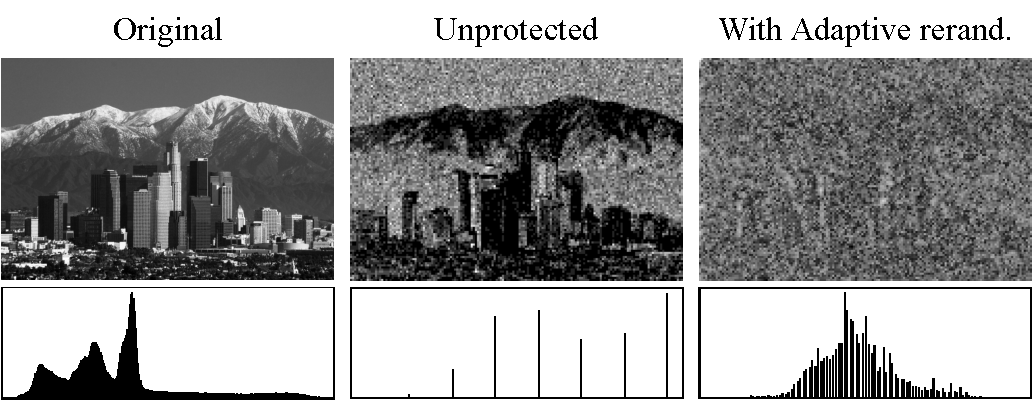
\includegraphics[width=0.95\columnwidth]{figures/incognitos/jpeg-attack.pdf}
	\end{center}
	\caption{Image extraction results on LibJPEG using NPF controlled-channel attack~\cite{xu2015controlledchannel} against unprotected Unikraft CVM vs. \thename. }
	%Distribution of image pixels is shown below each image.}
	\label{fig:jpeg-attack}
\end{figure}

\begin{table*}[h]
	\centering
	\scriptsize
	% \fontsize{7}{8}\selectfont
	% Shrink vertical
	\renewcommand{\arraystretch}{.4}
	% \setlength\extrarowheight{9pt}
	% \setlength{\aboverulesep}{0pt} % Space above \midrule
	% \setlength{\belowrulesep}{0pt} % Space below \midrule
	% Shrink horizontal
	\setlength\tabcolsep{4pt}
	
\begin{adjustbox}{angle=90}
	\begin{threeparttable}
    \begin{NiceTabular}{@{}>{\it }lll*{15}r@{}}[corners]
			% \cmidrule(){2-3} 
			\CodeBefore
			\rowlistcolors{4}{gray!8, }[cols=1-18]
			% \rowcolors[gray]{2}{0.8}{}[cols=2-3,restart]
			\Body
			\toprule
			\Block{3-1}{\thead{Bench.}} & \Block{2-2}{\thead{ReRand.                                                                                                                                                                         \\Disabled}}& &\Block{1-15}{\thead{Static Rerandomization}} &&&&&&&&&&&&&&\\
			\cmidrule(rl){4-18}
			% \cmidrule(rl){9-14}
			% \cmidrule(rl){15-17}

			~                           & ~                          & ~    &
			\Block{1-3}{\thead{$\freqrrof{Static}=$1/10K}}
			                            &                            &      & \Block{1-3}{\thead{$\freqrrof{Static}=$1/100K}}
			                            &                            &      & \Block{1-3}{\thead{$\freqrrof{Static}=$1/500K}}
			                            &                            &      & \Block{1-3}{\thead{$\freqrrof{Static}=$1/1M}}
			                            &                            &      & \Block{1-3}{\thead{$\freqrrof{Static}=$1/2M}}                                                                                                                  \\
			\cmidrule(rl){2-3}
			\cmidrule(rl){4-6}
			\cmidrule(rl){7-9}
			\cmidrule(rl){10-12}
			\cmidrule(rl){13-15}
			\cmidrule(rl){16-18}
			% \cmidrule(rl){8-11}
			% \cmidrule(rl){12-15}
			% \cmidrule(rl){4-7}
			% \cmidrule(rl){3-4}
			% \cmidrule(rl){5-6}
			% \cmidrule(rl){7-8}
			% \cmidrule(rl){9-11}
			% \cmidrule(rl){12-14}
			% \cmidrule(rl){15-17}
			~                           & \thead{Ovh.                                                                                                                                                                                        \\($\times$)} & \thead{\#Tick}
			                            & \thead{Ovh.                                                                                                                                                                                        \\($\times$)} & \thead{\#RR} & \thead{\#PF}
			                            & \thead{Ovh.                                                                                                                                                                                        \\($\times$)} & \thead{\#RR} & \thead{\#PF}
			                            & \thead{Ovh.                                                                                                                                                                                        \\($\times$)} & \thead{\#RR} & \thead{\#PF}
			                            & \thead{Ovh.                                                                                                                                                                                        \\($\times$)} & \thead{\#RR} & \thead{\#PF}
			                            & \thead{Ovh.                                                                                                                                                                                        \\($\times$)} & \thead{\#RR} & \thead{\#PF}
			\\
			\midrule
			NumSort                     & 3.29                       & 326M & 381.40                                          & 55K  & 5036.2  & 41.05  & 58K & 4537.6  & 14.60 & 44K & 2545.6 & 8.85  & 44K & 2099.6 & 7.92  & 33K & 1172.6 \\
			StrSort                     & 3.24                       & 313M & 327.93                                          & 55K  & 4591.8  & 39.12  & 49K & 3635    & 11.57 & 37K & 2450.6 & 8.09  & 29K & 1752.2 & 6.31  & 22K & 1122.6 \\
			Bitfield                    & 6.74                       & 411M & 186.96                                          & 53K  & 17216.6 & 30.30  & 38K & 10092.8 & 16.56 & 24K & 3643.4 & 13.96 & 20K & 2161.4 & 12.33 & 15K & 1218.6 \\
			EmFloat                     & 3.43                       & 291M & 477.88                                          & 113K & 11553.4 & 71.28  & 54K & 3989.8  & 19.41 & 40K & 2578.2 & 12.86 & 34K & 1914   & 9.46  & 28K & 1286.4 \\
			Fourier                     & 5.40                       & 289M & 1726.60                                         & 76K  & 3189.4  & 217.53 & 52K & 1758.4  & 53.16 & 44K & 1375   & 30.26 & 39K & 1199.2 & 18.64 & 32K & 973.6  \\
			Assign                      & 1.75                       & 179M & 182.40                                          & 55K  & 2598.2  & 20.44  & 53K & 2236.4  & 6.24  & 36K & 1404.2 & 4.25  & 27K & 1035   & 3.07  & 19K & 704.8  \\
			IDEA                        & 5.28                       & 327M & 434.82                                          & 90K  & 14955.8 & 46.40  & 54K & 8378.2  & 17.78 & 33K & 4189   & 12.58 & 24K & 2962   & 9.59  & 16K & 1944.8 \\
			Huffman                     & 3.63                       & 289M & 130.09                                          & 61K  & 10246.2 & 18.94  & 43K & 6149.8  & 8.15  & 25K & 2705.8 & 6.30  & 16K & 1742.4 & 5.33  & 10K & 1024.8 \\
			NNET                        & 2.25                       & 186M & 1106.01                                         & 111K & 4830.6  & 110.57 & 56K & 2431    & 24.84 & 45K & 1945.8 & 13.94 & 41K & 1741.6 & 8.24  & 35K & 1464.4 \\
			LU Dec.                     & 7.44                       & 354M & 1541.90                                         & 52K  & 2558.2  & 203.94 & 50K & 1885.8  & 53.91 & 44K & 1418.4 & 34.12 & 42K & 1118.6 & 24.02 & 40K & 794.4  \\
			% GEOMEAN&3.87&449.87&&&56.04&&&17.96&&&12.01&&&8.97&&\\
			% StrSort&3.85&469M&3339.44&11K&31K (29\%)&76K (71\%)&8.33&11K&17K (22\%)&58K (78\%)&5.13&991&7K (20\%)&28K (80\%)\\
			% Bitfield&9.61&585M&1375.22&49K&37K (38\%)&61K (62\%)&9.80&49K&27K (69\%)&12K (31\%)&10.88&858&10K (70\%)&4K (30\%)\\
			% EmFloat&3.80&454M&1943.78&90K&118K (41\%)&171K (59\%)&7.69&90K&33K (50\%)&33K (50\%)&4.93&443&8K (62\%)&5K (38\%)\\
			% Fourier&6.44&449M&9196.11&16K&95K (50\%)&95K (50\%)&14.36&16K&35K (43\%)&46K (57\%)&7.35&441&4K (36\%)&8K (64\%)\\
			% Assign&2.40&125M&868.66&26K&195K (85\%)&33K (15\%)&2.63&26K&37K (73\%)&13K (27\%)&3.18&2K&22K (73\%)&8K (27\%)\\
			% IDEA&6.08&223M&2853.28&74K&91K (35\%)&166K (65\%)&7.72&74K&21K (49\%)&21K (51\%)&7.14&479&2K (42\%)&2K (58\%)\\
			% Huffman&4.02&362M&799.09&51K&109K (63\%)&64K (37\%)&3.77&51K&20K (72\%)&8K (28\%)&5.03&2K&8K (69\%)&3K (31\%)\\
			% NNET&2.78&272M&4583.57&45K&189K (45\%)&227K (55\%)&6.64&45K&36K (43\%)&47K (57\%)&2.85&316&3K (35\%)&5K (65\%)\\
			% LU Dec.&8.08&505M&6604.33&12K&83K (83\%)&17K (17\%)&19.81&12K&71K (81\%)&16K (19\%)&9.53&2K&67K (79\%)&18K (21\%)\\
			\midrule
			GeoMeaBn                    & 3.87                       &      & 449.87                                          &      &         & 56.04  &     &         & 17.96 &     &        & 12.01 &     &        & 8.97  &     &        \\
			% GEOMEAN&4.65&&2494.71&&&&7.56&&&&5.58&&&\\
			\bottomrule
		\end{NiceTabular}
		\centering
		\caption{Performance overheads \textbf{\emph{Ovh.}} of different \thename configurations, compared against unmodified \nbench execution.
			Average number of executed synchronous ticks (\textbf{\emph{\#Tick}}), page faults (\emph{\textbf{\#PF}}) and rate-adaptive rerandomizations (\emph{\textbf{\#RR}}) for each benchmark iteration are also reported. Number of synchronous ticks remains mostly constant across settings.}\label{tab:nbench}
	\end{threeparttable}
\end{adjustbox}

\end{table*}

\hdr{Result discussion}
Without \thename's protection, the attack can reconstruct the patterns of the compressed image with minimal noise (the \emph{Unprotected} image).
% Specifically, we found that $7$ \limcomm{hard to understand what the pixel value is}{distinct pixel values} based on the access count can be deterministically extracted.
On the other hand, the constant page rerandomizations (about eight times per extracted pixel) render most of the extracted features unrecognizable (\emph{With Adaptive rerand.} image).
Also, the distribution of extracted pixel values (shown as a histogram under the image) becomes smooth because of this.
% \limcomm{Too long. Brief explanation is enough.}{
% This is because the locations of the physical pages in the active region are constantly rerandomized throughout the attack, rendering the access counts on each attacker-observable location meaningless.
% }
% During this attack, an average VMExit rate of \textcolor{red}{XXX} was measured, resulting in    \textcolor{red}{(??)}.





% \subsection{Performance evaluation}
% We evaluated \thename's performance using the \texttt{nbench}~\cite{nbench} benchmark suite microbenchmarks and two real-world workloads: NGINX and Redis.


\begin{figure}[t]
	\centering
	% \scriptsize
	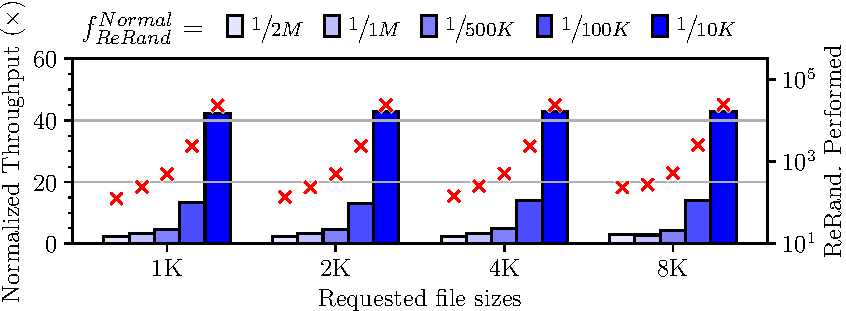
\includegraphics[width=0.95\columnwidth]{figures/incognitos/nginx}
	\caption{Throughput of \thename-hosted NGINX web server with varied requested file sizes and rerandomization frequency, normalized to the throughput of baseline NGINX Unikraft.
		\textcolor{red}{\bfseries $\times$} marks number of rerandomizations performed.} \label{tab:nginx}
\end{figure}
% , similar to previous works on side-channel defenses~\cite{zhang2020klotski, brasser2019drsgx, shih2017tsgx, seo2017sgxshield}.
\subsection{nbench microbenchmark}
\label{sec:eval:microbench}
We illustrate the performance characteristics of \thename using the \nbench~\cite{nbench} benchmark.
The results are shown in \autoref{tab:nbench}.

\hdr{Experiment setup}
We deployed different configurations of \thename-hosted \nbench.
The \emph{ReRand. Disabled} column shows the benchmark results with the synchronous tick instrumentation but \emph{without} rerandomization, thereby illustrating the isolated overhead from the ticks.
We also illustrate the performance overhead of \thename's rerandomization in varied \emph{static} frequency of $\freqrrofof{ReRand}{Static}=$1/\{10K, 100K, 500K, 1M, 2M\}.
While \thename uses rate-adaptive rerandomization in practice, the static frequencies allow us to understand the security and performance tradeoffs when configuring the policy parameters (e.g., $\freqrrof{Normal}$).
% While \thename applies a rate-adaptive policy, these results allow us to estimate the overhead and understand the security and performance tradeoffs necessary for configuring the policy parameters (e.g., $\freqrrof{Normal}$).
% \limcomm{Why is this sentence here?}{With no side-channel attack, we found that none of the benchmarks in the suite experienced an alarmed state.}
For each configuration, we ran the benchmark for fixed $1,000$ iterations and took the average for the statistics of each run.

% and compared the built-in scores with the unprotected Unikraft \nbench score.

% and columns show  \textbf{\emph{Ovh.}}, \textbf{\emph{\#Tick}}, \textbf{\emph{\#RR}} and \textbf{\emph{\#PF}}

%     We identify the main overhead sources for \thename during normal program execution: (1) the execution of synchronous ticks and (2) runtime rerandomization, which leads to additional page faults due to evicting pages from the active regions.
% }

\hdr{Result discussion: isolated tick overhead}
The results show an average performance degradation of $3.87\times$ for the \nbench suite.
Since \thename performs per basic block synchronous tick placement, the total number of tick triggered varies across different programs.
The number of synchronous ticks executed (\emph{\#Tick}) in each program in the suit illustrates how the overheads generally scale with the number of ticks.
The most significant slowdown occurs in \texttt{LU Decomposition} (7.44$\times$, 354M tick executions), while the least slowdown is in \texttt{Assign} (1.75$\times$, 179M).



\hdr{Result discussion: performance impact of rerandomization frequency}
Understandably, the rerandomization was a major source of overhead; the geometric mean of overhead in the benchmarks was lowest (8.97$\times$) when the rerandomization frequency was at 1/2M and highest when at 1/10K (449.87$\times$).
Different benchmarks responded differently to the varied rerandomization rate due to two likely sources.
The first is the size of the working set pages for each benchmark, which affects the number of page faults between each rerandomization.
The second is the instruction accumulation rate (proportional to the basic block sizes and number of executed instructions), which impacts the number of rerandomizations.
% This rate is determined by the basic block sizes in each program and the number of executed instructions per iteration.
% \texttt{LU Decomposition} and \texttt{Fourier} consistently displayed the highest overheads among \nbench, with $1541.9\times$ and $1726.60\times$ in the worst case ($\periodrrof{Static} = 10$K) and $24.02\times$ and $18.64\times$ in the best case ($\periodrrof{Static} = 2$M).


% The impact of rerandomization is particularly high on benchmarks with large working sets of pages, likely due to the complete eviction scheme for rerandomization.
% For instance, with the highest \freqrrof{Static} of 2M, overheads of  $18.64\times$ for Fourier and $24.02 \times$ for LU Decomposition are observed. 
% Throughout the execution of \nbench, the measured exit rate does not exceed the configured \freqvmexitof{Alarm} (which might not apply to networking workloads).
% Thus, the configurable \freqrrof{Normal} is the other factor that contributes to the overheads.
% The results in \autoref{tab:nbench} show the performance overheads of adaptive rerandomization, which improve as \freqrrof{Normal} increases. 


% To study the performance impact of \freqvmexitof{Alarm}, we run \nbench with the adaptive rerandomization scheme enabled (\textbf{Adaptive Rerandomization}) while varying the \freqrrof{Normal} parameters with the value range discussed in \cref{subsec:policy-parameters}.


% With a relatively relaxed \freqrrof{Normal} of 2M, an average performance overhead of $8.97$ times is observed.


\iffalse
	\hdr{Performance of ORAM-backed paging}
	We also evaluated the isolated performance overhead from \thename's ORAM-backed paging subsystem.
	We select small active \gls{gpa} region sizes ($A=8$, 16, and 64) to trigger frequent random evictions and ORAM fetches throughout the benchmarks.
	The results indicate moderate overheads may be observed in active region sizes smaller than the working set, as indicated by a large amount of page faults observed when A=8.
	Larger active region sizes encompassing the benchmark working set (e.g., $A=64$) allow the paging subsystem to approach baseline execution.
	This is particularly due to the lack of memory access instrumentation per memory access like previous obfuscated execution engines~\cite{obelix,zhang2020klotski,ahmad2019obfuscuro}, allowing native memory accesses when the pages are mapped.
\fi



% \begin{figure*}



% \hfill




\subsection{Real-world application performance}
\label{sec:eval:real-app}
We evaluate the performance of \thename with two unmodified real-world applications built for Unikraft~\cite{unikraft-dynamic-app}, the NGINX web server, and Redis in-memory key-value store.
% We deployed the applications into unmodified Unikraft instances and \thename instances with increasing configured \freqrrof{Normal}.
The results are presented in \autoref{tab:nginx} and \autoref{tab:redis}.

\hdr{Experiment setup} For both NGINX and Redis, we applied intensive workloads using each program's benchmark tools.
However, no side-channel attack was applied during the benchmark.
Also, we enabled \thename's adaptive rerandomization with varied \freqrrof{Normal}. This means that the short-lived rerandomization rate spikes are expected during execution.
All throughput measurements are normalized to those of vanilla Unikraft running inside a CVM.
% Based on the results in \cref{sec:eval:microbench},


% Also, two different active \gls{gpa} region sizes were employed, $A=512$ pages (2MB) and $A=1024$ pages (4MB) per code and data regions.

% \begin{table}[t]
%   \scriptsize
%   % \setlength\tabcolsep{4pt}
%  \begin{NiceTabular}{@{}clrrrrrr}[corners]
%  % \cmidrule(){2-3} 
%  \CodeBefore
%  \rowlistcolors{3}{,gray!20}[cols=2-8]
% % \rowcolors[gray]{2}{0.8}{}[cols=2-3,restart]
% \Body
% \toprule
%     &\Block{2-1}{\thead{Max DB\\size\\(MB)}}& \Block{1-2}{\confbaseline} & \Block{1-4}{\confadaptive} &&& \\ 
%       \cmidrule(rl){3-4}
%       \cmidrule(rl){5-8}
%     && \thead{Throughput\\(req/s)} & \thead{CPU\\util. (\%)} & \thead{Relative th.\\(\%)} & \thead{\#RR} & \thead{\#PF} & \thead{CPU\\util. (\%)}\\
%      \midrule
%     \Block{4-1}<\rotate>{\thead{\texttt{LPUSH}}}
%     &x&x&X&X&X&x&x\\
%     &x&x&X&X&X&x&x\\
%     &x&x&X&X&X&x&x\\
%     &x&x&X&X&X&x&x\\
%     \midrule
%     \Block{4-1}<\rotate>{\thead{\texttt{GET}}}
%     &x&X&X&X&x&x&x\\
%     &x&X&X&X&x&x&x\\
%     &x&X&X&X&x&x&x\\
%     &x&X&X&X&x&x&x\\
     
%         \bottomrule
%     \end{NiceTabular}


\newcolumntype{R}{>{\raggedleft\arraybackslash}X}
% Shrink vertical
\renewcommand{\arraystretch}{.85}
% Shrink horizontal
% \setlength\tabcolsep{5.5pt}
\setlength\tabcolsep{4pt}
 \begin{NiceTabularX}{\columnwidth}{@{}cccrRRrRRr}[corners]
 % \cmidrule(){2-3} 
 \CodeBefore
 \rowlistcolors{4}{gray!20,}[cols=3-10]
% \rowcolors[gray]{2}{0.8}{}[cols=2-3,restart]
\Body
\toprule
    &\Block{3-2}{\thead{Max mem. sz \\\& Payload sz}} && \Block{3-1}{\thead{Unmodified\\Redis\\throughput\\(req/s)}} & \Block{1-6}{\thead{With adaptive rerandomization}} &&& \\ 
    \cmidrule(rl){5-10}
    &&&& \Block{1-3}{$A=512$} &&& \Block{1-3}{$A=1024$} &&\\ 
    
      \cmidrule(rl){5-7}
      \cmidrule(rl){8-10}
      % \cmidrule(rl){4-7}
    &&&& \thead{Ovh.\\($\times$)} & \thead{\#RR} & \thead{\#PF}  & \thead{Ovh.\\($\times$)} & \thead{\#RR} & \thead{\#PF}  \\
     \midrule
     % &&\\
    \Block{4-1}<\rotate>{\thead{\texttt{LPUSH}}}
    & \Block{2-1}{8MB}  & 4KB&
        2930.83 & 3.35 & 205 & 110K & 2.62 & 205 & 83K \\ 
    && 8KB&
        1337.79 & 2.85 & 402 & 144K & 2.23 & 401 & 121K \\ 
    &\Block{2-1}{64MB}  & 4KB&
        2949.85 & 3.52 & 206 & 111K & 2.76 & 206 & 83K \\ 
    && 8KB&
        1336.18 & 2.95 & 401 & 147K & 2.31 & 403 & 122K \\ 
        \midrule
    \Block{4-1}<\rotate>{\thead{\texttt{GET}}}
    & \Block{2-1}{8MB}  & 4KB&
        6863.42 & 3.89 & 200 & 38K & 2.56 & 200 & 32K \\ 
    & & 8KB&
        6297.23 & 3.36 & 201 & 38K & 2.33 & 200 & 31K \\ 
    & \Block{2-1}{64MB}  & 4KB&
        7087.17 & 3.44 & 201 & 38K & 2.77 & 200 & 32K \\ 
    & & 8KB&
        6715.92 & 3.91 & 200 & 40K & 2.65 & 200 & 33K \\
    \midrule
    &\Block{1-2}{\textbf{GEOMEAN}}&&
        ~ & 3.39 & ~ & ~ & 2.52 & ~ & ~ \\[-.6em]
         
%     \midrule
%     \Block{4-1}<\rotate>{\thead{{Concurr.}}} & 1K
%     & 156.66 & 3.84 & 34 & 236K & 1.26 & 45 & 17K \\ 
%         ~ & 2K & 154.95 & 2.42 & 47 & 119K & 1.26 & 45 & 18K \\ 
%         ~ & 4K & 152.30 & 2.32 & 48 & 114K & 1.28 & 49 & 19K \\ 
%         ~ & 8K & 153.89 & 3.35 & 42 & 205K & 1.26 & 43 & 16K \\ 
%     \midrule
% &    &    \textbf{GEOMEAN} & ~ & 3.95 & ~ & ~ & 1.27 & ~ & ~ \\ 
    % \Block{4-1}<\rotate>{\thead{Single}}\\

    % \Block{4-1}<\rotate>{\thead{Concur.}}\\
     
        \bottomrule
    \end{NiceTabularX}
%   \caption{Througputh of Redis}\label{tab:redis}.
% \end{table}


\hdr{NGINX webserver}
We measured the throughput (i.e., HTTPS requests processed per second) of the \thename-hosted NGINX with the \emph{Apache Benchmark tool} (\texttt{ab})~\cite{apache-benchmark}.
% and compared it against that of the unmodified NGINX hosted on Unikraft.
The keepalive option (\texttt{-k}) was not applied, which makes each request perform a full connection establishment to evaluate the worst-case scenario.
We use \texttt{ab} to perform 1000 concurrent requests (\texttt{-c 8}) on the webserver to retrieve files with varied file sizes: 1KB, 2KB, 4KB, and 8 KB.
% Since Unikraft utilizes an in-memory file system (\texttt{vfscore}), the memory used for the requested file is covered by \thename's paging scheme, leading to in

% \khacomm{todo}{
% \lipsum[2-2]
% }

% \autoref{tab:nginx} shows the throughput 

\begin{figure}[t]
	\centering
	% \scriptsize
	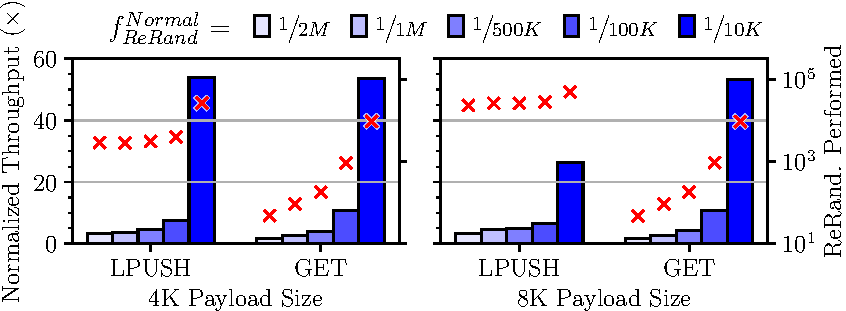
\includegraphics[width=0.95\columnwidth]{figures/incognitos/redis.pdf}
	\caption{
		Throughput of \thename-hosted Redis in back-to-back \texttt{LPUSH} and \texttt{GET} workloads with 4K and 8K payloads, normalized to throughput of baseline Redis on Unikraft.
		\textcolor{red}{\bfseries $\times$} marks number of rerandomizations performed.
	} \label{tab:redis}
\end{figure}
\hdr{Redis in-memory data store}
Similarly, we use \texttt{redis-benchmark}~\cite{redis-benchmark} to benchmark the performance of \thename-enabled Redis server.
We launched the Redis server with a storage size of 64MB.
We filled the server memory usage to its maximum using \texttt{LPUSH} for data storage, followed by a \texttt{GET} workload.
Each workload consisted of 10,000 requests, with payload sizes of 4KB and 8KB.
The benchmarking was set to use 50 parallel connections (\texttt{-c 50}) with TCP keepalive enabled (\texttt{-k}) and randomized access keys (\texttt{-r 10000}).
We obtained the throughput (commands served per second) and compared it against the throughput of an unmodified Redis workload deployed to Unikraft.
% the results of this evaluation are shown in \autoref{tab:redis}.

\hdr{Result discussion:} \freqrrof{Normal} and performance trade-off
We found that the configurable rerandomization frequency during benign execution \freqrrof{Normal} also closely correlated to the performance overheads of real-world applications, similar to the microbenchmark's performance characteristics.
Redis and NGINX both saw significant overheads with the smallest \freqrrof{Normal} of 1/10K, $42.67\times$ and $44.84\times$ on average for NGINX and Redis.
However, with a relaxed \freqrrof{Normal} of 1/2M, the performance overheads dropped to $2.45\times$ and $2.46\times$.
As shown throughout the security evaluation, this relaxed \freqrrof{Normal} would maintain resilience under attacks thanks to \thename's adaptive rerandomization policy.
More aggressive values for \freqrrof{Normal} may be chosen in anticipation of attacks with very low exit rates.

% do so without affecting robustness, while being more aggressive (we further discuss) in the next subsection.
% NOte that 
% This dramatic



% overhead drops to 

\iffalse
	The average performance overheads sharply decreased (down to $13.6\times$ and $8.55\times$) when the value increased to 1/100K and minimized ($2.45\times$ and $2.46\times$) on the lowest frequency 1/2M.

	An overall geometric mean of $7.31\times$ and $6.72\times$ is seen across all configurations of the two applications.
\fi
% The lower overheads compared to 
% This result aligns with the microbenchmark results discussed in \cref{sec:eval:microbench}. 
% However, we found that decreases in rerandomization rates are less impactful after certain \freqrrof{Normal} is reached.

\key{
	\hdr{Result discussion: performance loss from spikes}  The momentary benign spikes in VMExit frequencies were sparse throughout the performance evaluation and contributed minimally to the total overheads.
}
In particular, for NGINX and Redis, the \emph{maximum} number of ticks being in an alarmed state observed was $1798$ ($0.006\%$ of all ticks) during serving 8K files and  $1,347,282$ ($5.11\%$) during \texttt{LPUSH} with 8K payloads.
% In contrast, as we have seen in \cref{subsec:robustness-eval}, most ticks are in elevated rerandomization states during the attacks.
Note, we used the same \freqvmexitof{Alarm} threshold across the evaluations ($0.003$), and lower thresholds may be fine-tuned for a specific application to reduce the impacts of spikes further.
Based on this result, we conclude that \thename's rerandomization policy effectively suppresses obfuscation overheads.

